\documentclass[20pt,margin=1in,innermargin=-4.5in,blockverticalspace=-0.25in]{tikzposter}
\geometry{paperwidth=42in,paperheight=30in}
\usepackage[utf8]{inputenc}
\usepackage{csquotes}
% \usepackage[estonian]{babel}
\usepackage{amsmath}
\usepackage{amsfonts}
\usepackage{amsthm}
\usepackage{amssymb}
\usepackage{mathrsfs}
\usepackage{enumitem}
\usepackage{graphicx}
\usepackage{adjustbox}
\usepackage{xcolor}
\usepackage[backend=biber,style=numeric]{biblatex}
\usepackage{CIMAT}
%\usepackage{subfigure}

%Declarations
\newtheorem{theorem}{Teorema}[section]
\newtheorem*{proposition}{Proposici\'on}
\newtheorem{corollary}[theorem]{Corolario}
\newtheorem{lemma}[theorem]{Lema}
\newtheorem*{definition}{Definici\'on}
\newtheorem*{remark}{Observaci\'on}
\newtheorem*{ejemplo}{Ejemplo}
\newtheorem{claim}[theorem]{Claim}
\newtheorem{conjecture}[theorem]{Conjetura}
\newtheorem*{conjecture*}{Conjetura}
\newtheorem*{theorem*}{Teorema}
\newtheorem*{lemma*}{Lema}

\newcommand{\Aut}{\operatorname{Aut}\nolimits}
\newcommand{\alg}{\operatorname{Alg}\nolimits}
\newcommand{\sete}{\operatorname{Set}\nolimits}
\newcommand{\Coker}{\operatorname{Coker}\nolimits}
\newcommand{\colim}{\operatorname{colim}\nolimits}
\newcommand{\hocolim}{\operatorname{hocolim}\nolimits}
\newcommand{\Hom}{\operatorname{Hom}\nolimits}
\newcommand{\ide}{\operatorname{id}\nolimits}
\newcommand{\me}{\operatorname{m}\nolimits}
\newcommand{\Ind}{\operatorname{Ind}\nolimits}
\newcommand{\inv}{\operatorname{inv}\nolimits}
\newcommand{\Ima}{\operatorname{Im}\nolimits}
\newcommand{\Inj}{\operatorname{Inj}\nolimits}
\newcommand{\Inn}{\operatorname{Inn}\nolimits}
\newcommand{\Iso}{\operatorname{Iso}\nolimits}
\newcommand{\Ker}{\operatorname{Ker}\nolimits}
\newcommand{\Out}{\operatorname{Out}\nolimits}
\newcommand{\Syl}{\operatorname{Syl}\nolimits}
\newcommand{\Rep}{\operatorname{Rep}\nolimits}
\newcommand{\Res}{\operatorname{Res}\nolimits}
\newcommand{\Top}{\operatorname{Top}\nolimits}
\newcommand{\grup}{\operatorname{Grp}\nolimits}
\newcommand{\nat}{\operatorname{Nat}\nolimits}

\usepackage{mwe} % for placeholder images

\addbibresource{ref.bib}

% set theme parameters
\tikzposterlatexaffectionproofoff
\usetheme{CIMATTheme}
\usecolorstyle{CIMATStyle}

\usepackage[scaled]{helvet}
\renewcommand\familydefault{\sfdefault} 
\renewcommand{\vec}[1]{\bm{#1}}
\newcommand{\Tr}{\text{Tr}}
\usepackage[T1]{fontenc}

\title{Cuantificación de incertidumbre bayesiana aproximada en problemas inversos de ODE}
\author{\textbf{César Isaí García Cornejo} \& \textbf{José Andrés Christen Gracia} }

\institute{Centro de Investigaci\'on en Matem\'aticas, CIMAT, A.C. }
\titlegraphic{
\includegraphics[width=0.05\linewidth]{logoCIMAT.jpg}}

% begin document
\begin{document}
\maketitle
\centering
\begin{columns}
    \column{0.32}
    \block{Introducción}{
        
        En una amplia gama de disciplinas se utilizan modelos que pretenden describir algún fenómeno. La inmensa mayoría de estos son modelos matematicos, teniendo relaciones entre variables relacionadas por ecuaciones dependietes de ciertos parámetros. El tipo de modelos considerados son aquellos cuyas variables se pueden expresar ya sea en una forma funcional o en forma de ecuación diferencial ordinaria (ODE).

        \begin{center}
                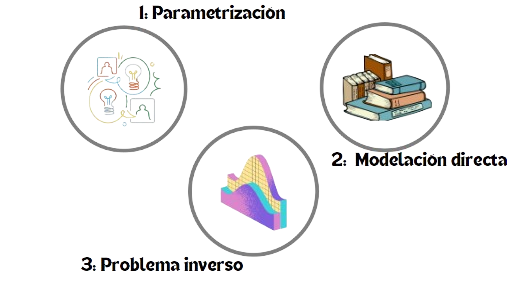
\includegraphics[width = 20 cm]{figuras/Modelos.png} 
        \end{center}
       

        El tratamiento del \textbf{problema inverso} se aborda con estadística bayesiana sobre los parámetros. Nos interesa cuantificar la incertidumbre de los parámetros dada una muestra del modelo de interés. La metodología usual considera muestrear de la distribución posterior de los parámetros con MCMC. El inconveniente de usar algoritmos de MCMC es que a cada paso que da la cadena, se debe de calcular una solución numérica de la ODE del modelo, que para modelos suficientemente complejos puede tardar una considerable cantidad de tiempo para obtener la cuantificación de la incertidumbre deseada. Es aquí que la trascendencia del proyecto radica en obtener una \textbf{propuesta aproximada de la distribución posterior} siguiendo cierta discretización de los parámetros. Donde se buscarán criterios para la convergencia de la posterior aproximada a la posterior teórica.
    }
         
    \block{Antecedentes}{

        El problema directo consiste en obtener trayectorias de observables que corresponde a un modelo con parámetros $\theta = (\theta_1,\theta_2,\cdots,\theta_d)$
        \begin{align*}
            \theta \mapsto y(t) = F(\theta)
        \end{align*}
        donde el modelo para la observable $y(t)$ se considera que satisface
        % \begin{align*}
        %     \frac{d y(t)}{dt} = f \left(\theta,t,y,\frac{dy}{dt},\cdots,\frac{d^my}{dt^m} \right) 
        % \end{align*}
        una ecuación diferencial ordinaria. Decimos que $F(\theta)$ es el \textit{forward map} del modelo.
        Consideremos que tenemos una muestra $y_i$ a ciertos tiempos $t_i$ denotada por $\mathbf{y} = (y_1,y_2,...,y_n)$.
        
        \begin{center}
            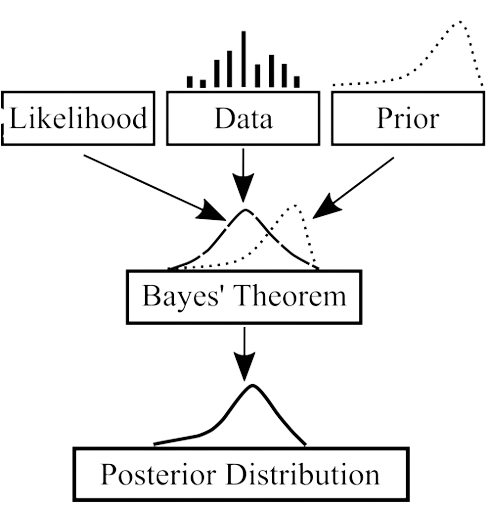
\includegraphics[width = 13 cm ]{figuras/bayes1.png} 
        \end{center}
        }	
        
        \column{0.32}

        
    \block{Forward Map Aproximado}{
            
        Salvo una constante, la distribución posterior con el forward map ordinario es 
        \begin{align*}
            \pi(\theta, \sigma|\mathbf{y}) \propto \left(\frac{1}{2\pi \sigma^2}\right) ^{n/2}\exp \left \{  -\frac{1}{2\sigma^2}\sum_{i = 1}^{n} \left(y_i - F_{\theta}(t_i)\right)^2 \right \} \pi(\theta)
        \end{align*}
        Sin embargo, se propone un forward map aproximado $F_{\theta}^{*}(t)$ de forma que dependa simplemente de una vecindad de los $n$ vecinos más cercanos.

        \begin{center}
            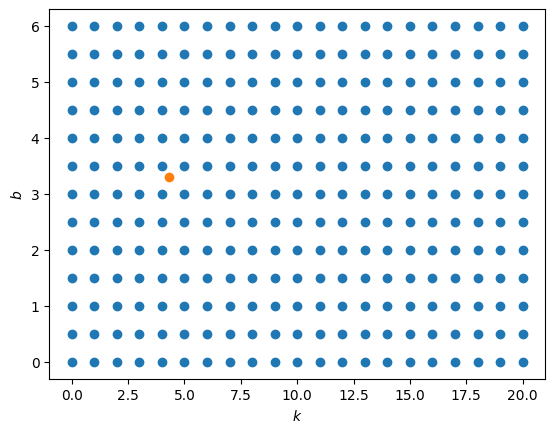
\includegraphics[width = 15cm]{figuras/5.png}
        \end{center}

        Además, es claro que para un vecino cercano $F^{*}_{\theta}\rightarrow F_{\theta}$ a medida que la malla se hace más fina.

        \vspace*{1cm}
    }
    
    
    
    \block{Experimentación}{

        \vspace{-0.8cm}
        \begin{center}
            \Large{\textbf{Modelo gravitatorio}}
        \end{center}
        \vspace{0.5ex}\hrule 

        \vspace*{1ex}

        Para el modelo de \textbf{caída gravitatoria sujeto a fricción}, la trayectoria es la distancia recorrida $x(t)$ dado por
        \begin{align*}
            m \ddot{x} = mg - b\dot{x}
        \end{align*}
        donde $g,b$ son parámetros del modelo. Con la distribución a priori $\theta_i \sim Gamma(\alpha_i,\theta_i^{*}/\alpha_i)$ para todo $i = 1,...,d$.

        \begin{center}
            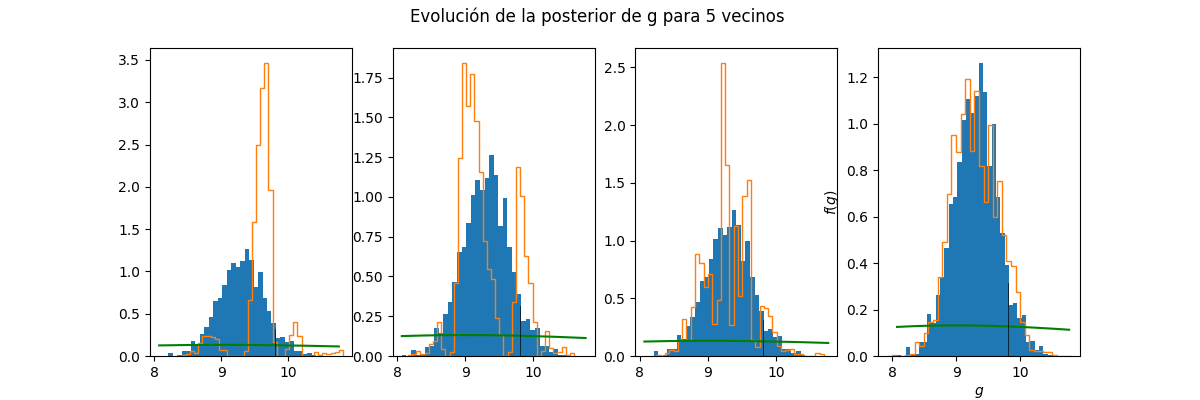
\includegraphics[width = 30 cm]{figuras/Convergencia_theta1_1_gravedad_sigma.png}
            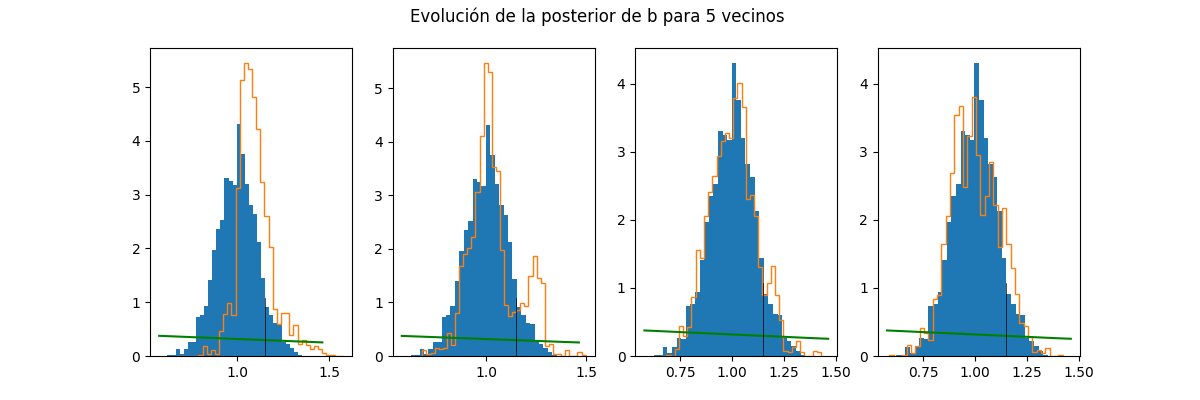
\includegraphics[width = 30 cm]{figuras/Convergencia_theta2_1_gravedad_sigma.png}
        \end{center}


    }


    
    \column{0.32}
    \block{}{
        
        \vspace{-0.8cm}
        \begin{center}
            \Large{\textbf{Modelo logístico}}
        \end{center}
        \vspace{0.5ex}\hrule 

        \vspace*{1ex}

        El modelo \textbf{logístico} describe el crecimiento poblacional a lo largo del tiempo
        \begin{align*}
            \frac{X(t)}{dt} = \theta_1 X\left(\theta_2 - X\right) 
        \end{align*}


        \begin{center}
            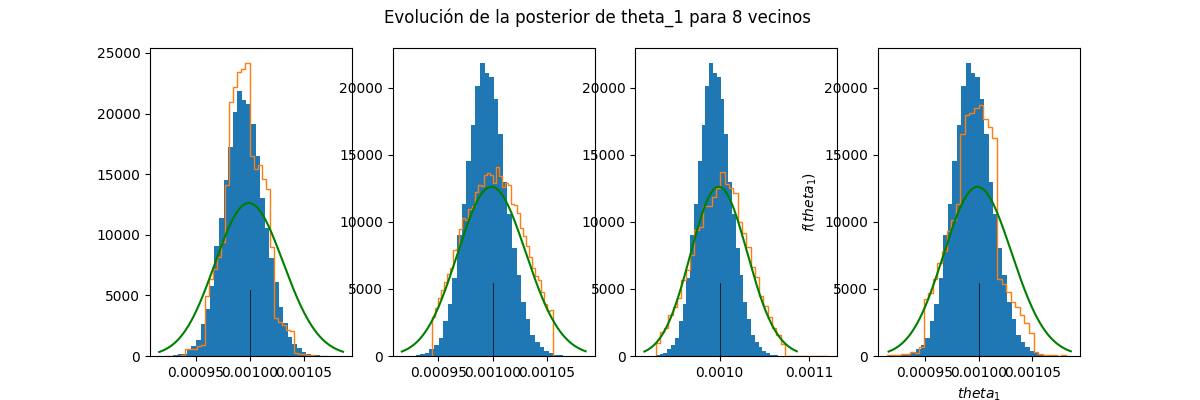
\includegraphics[width = 30 cm]{figuras/Convergencia_theta1_2_logistico_sigma.png}
            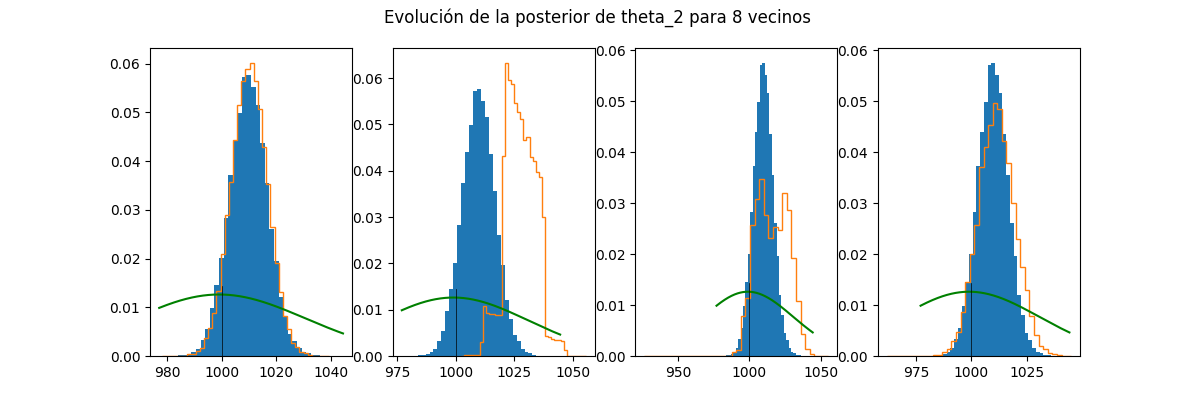
\includegraphics[width = 30 cm]{figuras/Convergencia_theta2_2_logistico_sigma.png}
        \end{center}




        \vspace{-0.8cm}
        \begin{center}
            \Large{\textbf{Modelo epidemiológico}}
        \end{center}
        \vspace{0.5ex}\hrule 

        \vspace*{1ex}








        Para el modelo \textbf{epidemiológico SIR} la cantidad de susceptibles, infectados y recuperados se rige por
        \begin{align}
            \frac{dS}{dt} &= -\beta S I \nonumber \\
            \frac{dI}{dt} &= \beta S I - \gamma I\\
            \frac{dR}{dt} &= \gamma I \nonumber
        \end{align}

        \begin{center}
            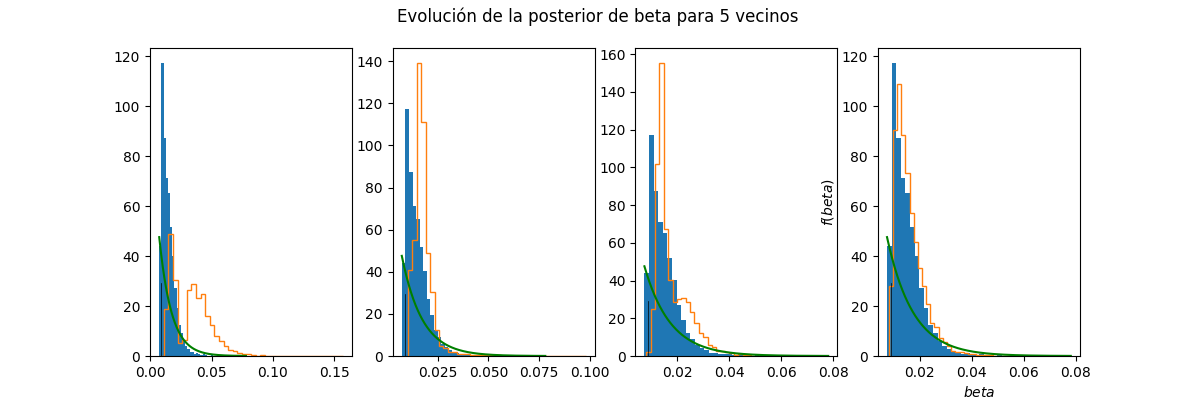
\includegraphics[width = 30 cm]{figuras/Convergencia_theta1_1_SIR_sigma.png} 
            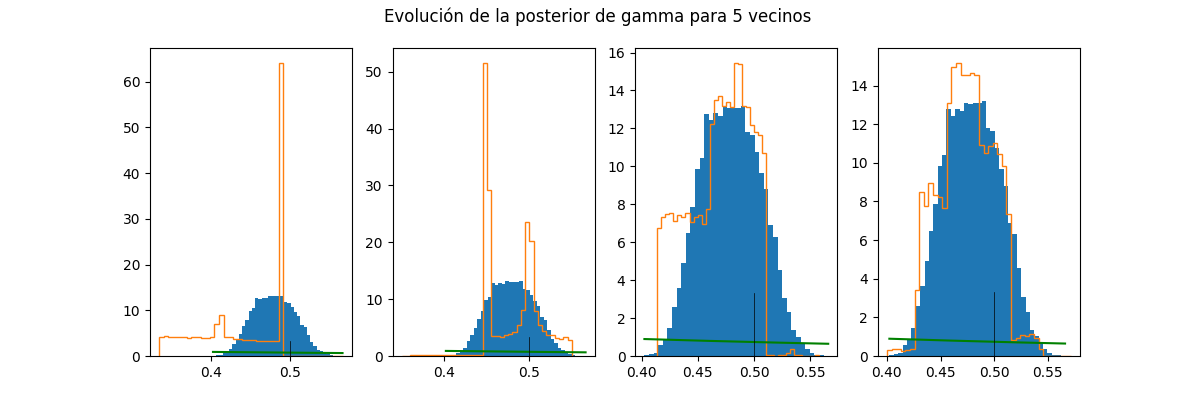
\includegraphics[width = 30 cm]{figuras/Convergencia_theta2_1_SIR_sigma.png}
        \end{center}










    }
    
    % \vspace{-0.1cm}
    % \block{References}{
    %     \vspace{-1em}
    %     \begin{footnotesize}
    %     \printbibliography[heading=none]
    %     \end{footnotesize}
    % }
    
\end{columns}
\end{document}